\documentclass[landscape,a1paper, fontscale=0.35]{baposter}
\usepackage[linesnumbered,ruled,vlined]{algorithm2e}
\SetAlFnt{\footnotesize}
\SetAlgoLined
\SetAlCapFnt{\small}
\SetAlCapNameFnt{\small}
\setlength{\algomargin}{1em}
\usepackage{tikz}
\usepackage{graphicx}
\usepackage{caption}
\usepackage{lettrine}
\usepackage{subcaption}
\usepackage{palatino}
\usetikzlibrary{shapes,arrows,positioning,calc}

%%%%%%%%%%%%%%%%%%%%%%%%%%%%%%%%%%%%%%%%%%%%%%%%%%%%%%%%%%%%%%%%%%%%%%%%%%%%%%%%
% Save space in lists. Use this after the opening of the list
%%%%%%%%%%%%%%%%%%%%%%%%%%%%%%%%%%%%%%%%%%%%%%%%%%%%%%%%%%%%%%%%%%%%%%%%%%%%%%%%
\newcommand{\compresslist}{%
\setlength{\itemsep}{1pt}%
\setlength{\parskip}{0pt}%
\setlength{\parsep}{0pt}%
}

\newcommand{\clustertriangle}{%
    \begin{center}
    \vspace{1em}
    \begin{tikzpicture}
        \node (spiderman) at (3,2)
        {\pgfbox[center, bottom]
            {\pgftext{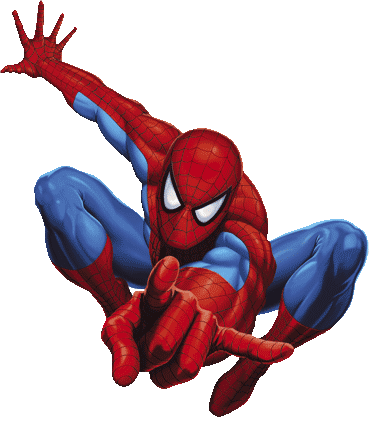
\includegraphics[height=5em]{images/spiderman.png}}}};
            \node (wolverine) at (1, 0)
        {\pgfbox[center, bottom]
            {\pgftext{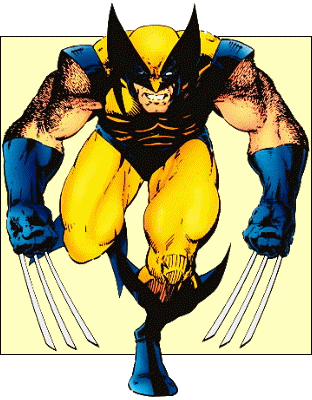
\includegraphics[height=5em]{images/wolverine.png}}}};
        \node (modok) at (5, 0)
        {\pgfbox[center, bottom]
            {\pgftext{
\includegraphics[height=5em]{images/modok.png}}}};
            \draw[-, dotted] (spiderman) -- node {link} (wolverine);
            \draw[-, dotted] (wolverine) -- node {link} (modok);
            \draw[-, dotted] (modok)     -- node {?} (spiderman);
    \end{tikzpicture}
    \vspace{1em}
\end{center}
}

\newcommand{\roulette}{%
\begin{tikzpicture}[scale=3]
    \vspace{1em}
\draw[dashed] (0cm, 0cm) circle(1cm);
\foreach \x/\y/\xcolour/\xopacity/\ximage/\xz/\xsize in {
    0/90/blue/0.5/spiderman/45/6em,
    280/360/blue/0.4/wolverine/310/5em,
    280/210/blue/0.3/modok/240/4em,
    210/140/blue/0.25/doom/180/4em,
    140/110/blue/0.2/ironman/120/2.5em,
    110/100/blue/0.15/hulk/100/2em,
    100/90/blue/0.1/thing/95/1em}
{
\filldraw[fill=\xcolour,draw=black, fill opacity=\xopacity](0:0cm) -- (\x:1cm)
arc (\x:\y:1cm) -- cycle;
\draw (\xz:0.6cm) node (\ximage) {\pgfbox[center, bottom]{
    \pgftext{\includegraphics[height=\xsize]{images/\ximage}}}};
}

\end{tikzpicture}
}

\newcommand{\approximation}{%
    \begin{minipage}[t]{0.45\textwidth}
            \vspace{0pt}
            \centering
        \begin{algorithm}[H]
            \SetAlgoLined
            \KwIn{Integer $k$ and a graph $G = \left(V,E\right)$ with $N$ nodes}
            \KwOut{An approximation of the clustering coefficient $C$ of $G$}
            $c \gets 0$\\
            \For{$i \in k$}
            {
            $j \gets\mathtt{\small UniformRandomNode}\left(\right)$\\
            $u \gets\mathtt{\small UnifromRandomNeighbour}\left(j\right)$\\
            \Repeat{$u \neq v$}
            {
                $v \gets \mathtt{\small UniformRandomNeighbour}\left(u\right)$\\
            }
            \If{$\mathtt{\small EdgeExists}\left(i, v\right)$}
            {
                $c \gets c + 1$\\
            }
            }%
            \KwRet{$c / k$}%
            \caption{Schank-Wagner}%
        \end{algorithm}%
    \end{minipage}%
}

\newcommand{\iterator}{%
    \begin{minipage}[t]{0.45\textwidth}
        \vspace{0pt}
        \centering
\begin{algorithm}[H]
\SetAlgoLined
                \KwIn{A graph $G = (V, E)$, with $N$ nodes}
                \KwOut{The clustering coefficient $C$, for $G$}
                $c \gets 0$\\
                \For{$i \in V$}
                {
                    $d \gets i.degree$\\
                    $e \gets 0$\\
                    \For{$j \in i.neighbours$}
                    {
                        \For{$k \in j.neighbours$}
                        {
                            \If {$i\mathtt{isneighbour}\left(i,j\right)$}
                            {
                                $e \gets e + 1$
                            }
                        }
                    }
                    $c \gets e / \left(d\left(d-1\right)\right)$
                }%
                \KwRet{$c / N $}%
                \caption{NODE-ITERATOR}%
            \end{algorithm}%
        \end{minipage}%
        }
\begin{document}
\definecolor{lightblue}{rgb}{0.145,0.6666,1}
\begin{poster}
    % Poster options
    {
        background=plain,
        bgColorOne=white,
        bgColorTwo=white,
        borderColor=lightblue,
        headerColorOne=blue,
        headerColorTwo=lightblue,
        headerFontColor=white,
        boxColorOne=white,
        boxColorTwo=lightblue,
        eyecatcher=true,
        headerborder=closed,
        headerheight=0.13\textheight,
      headerborder=closed,
      textfont={\setlength{\parindent}{1.5em}}
    }
{
    
\includegraphics[height=3.0em]{images/marvel.png}
}
{
    \LARGE Computing the Clustering Coefficient in Scale-free Networks
}
{
    Yegor Guskov, Lloyd Henning, Jacobus Meulen, Peter Sutton\\
    {\small\tt\{guskov9, henninl8, meulen9, suttonp8\}@cs.man.ac.uk}
}
{
    
\includegraphics[height=3.0em]{images/logo}
}
%%%%%%%%%%%%%%%%%%%%%%%%%%%%%%%%%%%%%%%%%%%%%%%%%%%%%%%%%%%%%%%%%%%%%%%%%%%%%%%
% Content begins
%%%%%%%%%%%%%%%%%%%%%%%%%%%%%%%%%%%%%%%%%%%%%%%%%%%%%%%%%%%%%%%%%%%%%%%%%%%%%%%
\headerbox{Problem}{name=problem,column=0,row=0}
{
    \lettrine{W}{e} present methods of computing the clustering coefficient of a
    Scale-free network to measure how clustered the nodes are.

}
%%%%%%%%%%%%%%%%%%%%%%%%%%%%%%%%%%%%%%%%%%%%%%%%%%%%%%%%%%%%%%%%%%%%%%%%%%%%%%%
\headerbox{Clustering Coefficient}{name=clustering, column=0, below=problem}
{
    \lettrine{G}{iven} a network $N = \left(V, E\right)$ and links $\left(u, v\right),
    \left(v, w\right) \in E$, the clustering coefficient $C_{N}$ gives the
    probability of there existing $\left(u, w\right) \in E$.

    Intuitively, we can understand it as: ``If Spiderman has appeared in the
    same comic as Wolverine and Wolverine has appeared in the same comic as
    M.O.D.O.K., what is the probability that Spiderman and M.O.D.O.K. have
    appeared in the same comic?''.
    \clustertriangle
    We define $C_{N}$ as
    \[
        C_{N} = \frac{1}{N} \displaystyle\sum_{i \in
        N}{2\frac{e}{k_{i}\left(k_{i} -1\right)}}
    \]
    Where $k$ is the number of neighbours of the $i^{th}$ node and $e$ is the
    number of links shared between them.
}
%%%%%%%%%%%%%%%%%%%%%%%%%%%%%%%%%%%%%%%%%%%%%%%%%%%%%%%%%%%%%%%%%%%%%%%%%%%%%%
\headerbox{BA model}{name=bamodel, column=1, row=0}
{
    \lettrine{S}{cale}-free networks can be emulated using the
    Barab\'{a}si-Albert (BA) model which grows the network through the addition
    of new nodes and preferring to attach new nodes old nodes with the highest
    degrees.

    The steps to generate a BA model are as follows
    \begin{enumerate}
    \compresslist
    \item
    Start with a random network $N$ composed of a small number of nodes.
    \item
        For each timestep $t \leq T$ add a new node $n$ to the graph and links
        $\left(n, i\right)$ where $i$ has degree $k_{i}$ and is selected from the
        existing nodes with probability
        \[
        \Pi\left(k_{i}\right) =
        \frac{k_{i}}{\displaystyle\sum_{j}{k_{j}}}
    \]
    \end{enumerate}

    \emph{Preferential attachment} is best seen as a ``roulette wheel'', where
    the nodes with greater degrees have more ``slots'' to land in.\\

    \noindent\roulette
}

%%%%%%%%%%%%%%%%%%%%%%%%%%%%%%%%%%%%%%%%%%%%%%%%%%%%%%%%%%%%%%%%%%%%%%%%%%%%%%
\headerbox{Experimental Results}{name=results, column=2, span=2, row=0}
{
    \begin{center}
        \begin{minipage}[t]{1\textwidth}
    \begin{minipage}[t]{0.49\textwidth}
        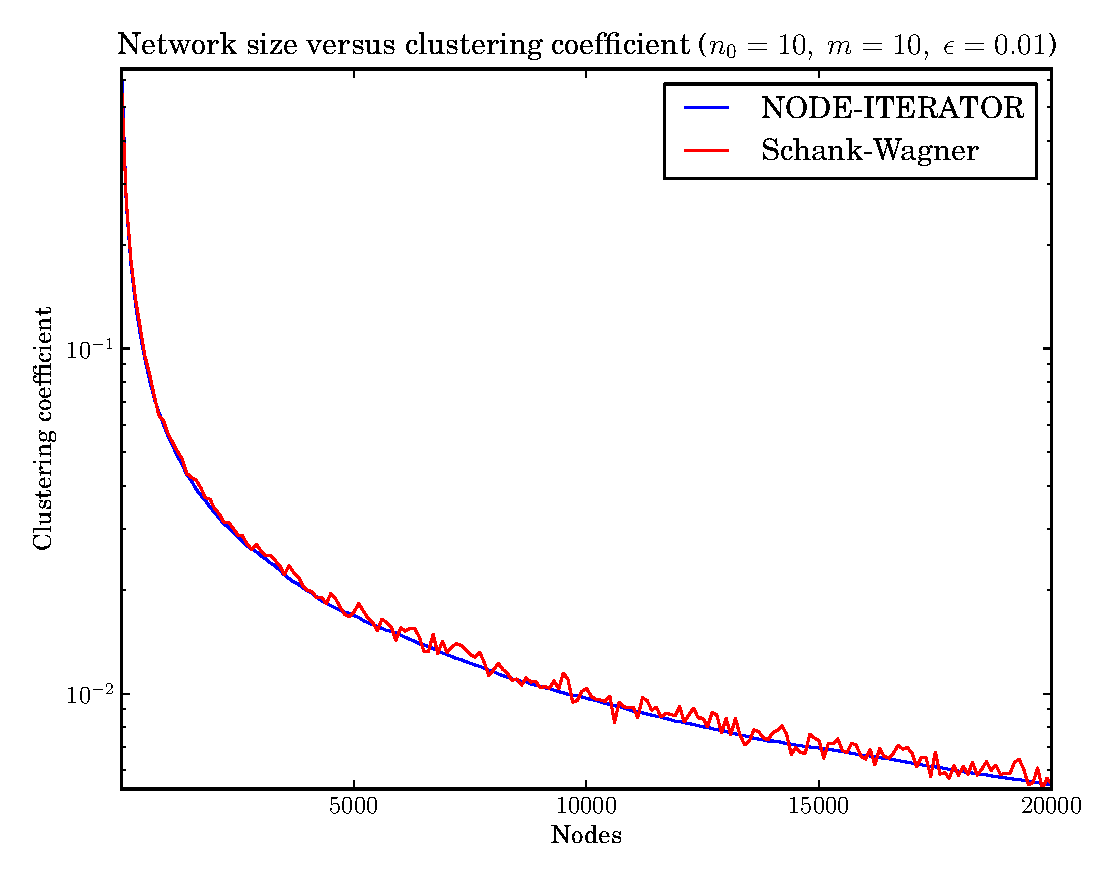
\includegraphics[height=15em]{images/cc.eps}
        \captionof{subfigure}[a]{\footnotesize Clustering coefficient}
    \end{minipage}
    \null
    \hfill
    \null
    \begin{minipage}[t]{0.49\textwidth}
        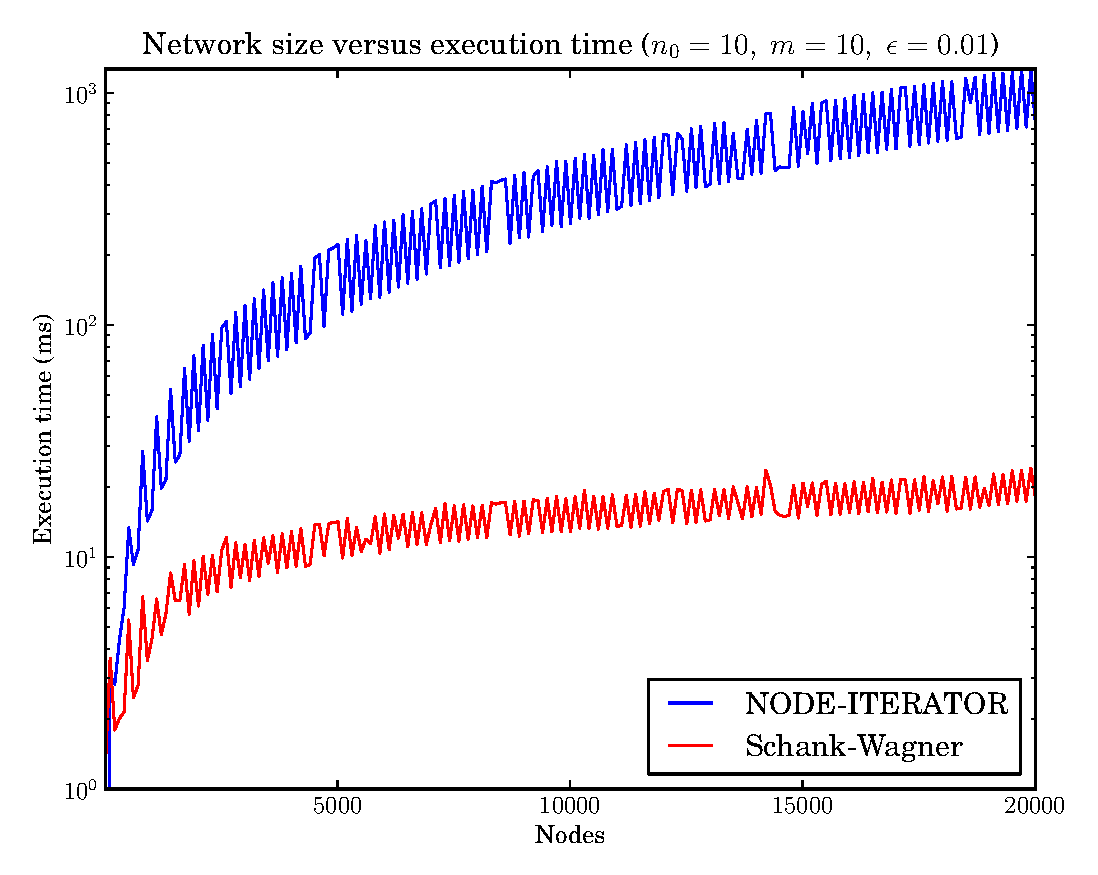
\includegraphics[height=15em]{images/time.eps}
        \captionof{subfigure}[b]{\footnotesize Execution time}
    \end{minipage}
    \hfill
    \null
    \captionof{figure}{\footnotesize Plots showing the performance of the
        exact NODE-ITERATOR and the approximate Schank-Wagner algorithms on
        networks generated by the BA model.}
    \end{minipage}
\end{center}
}
%%%%%%%%%%%%%%%%%%%%%%%%%%%%%%%%%%%%%%%%%%%%%%%%%%%%%%%%%%%%%%%%%%%%%%%%%%%%%%
\headerbox{Polynomial vs. Sublinear approaches}{name=exact-algorithm,
below=results ,column=2,span=2}
{
    \vspace{-1em}
    \null\hspace{-1em}
    \iterator\hspace{1em}
    \approximation
    \null\hfill\\
    \captionof{figure}{\footnotesize For a network of $n$ nodes, with $k_{max}$ as the
    largest degree of node, NODE-ITERATOR is $\mathcal{O}\left(nd^{2}\right)$
    and Schank-Wagner is $\mathcal{O}\left(k\right)$ where $k =
    \left(ln\left(2n\right)/2\epsilon^{2}\right)$ and $\epsilon$ is the error
        tolerated.}
    \label{cc-algorithms}%
}
%%%%%%%%%%%%%%%%%%%%%%%%%%%%%%%%%%%%%%%%%%%%%%%%%%%%%%%%%%%%%%%%%%%%%%%%%%%%%%
\headerbox{References}{name=references, column=0, below=clustering, above=bottom}
{
    \tiny
    \bibliographystyle{ieee}
    \renewcommand\refname{\vskip -0.5em}
    \begin{thebibliography}{1}
        \bibitem{Albert01:statisticalmechanics}
            R. Z. Albert and A. Barab\'{a}si
            \newblock{Statistical Mechanics Of Complex Networks},
            \newblock In {Reviews of Modern Physics, 2002, volume 74, page 47}
        \bibitem{Schank05:approximatingclustering}
            T. Schank, D. Wagner.
            \newblock {Approximating clustering coefficient and
                        transitivity}
                        \newblock In {Journal of Graph Algorithms and
                        Applications, 2005, volume 9, page 2005}
    \end{thebibliography}
}
\end{poster}
\end{document}
